\documentclass{beamer}
\usepackage{amsmath}
\usepackage{graphicx}
\usepackage{subcaption}
\usepackage{todonotes}
\usepackage{physics}
\usepackage{booktabs}
\usepackage[
    backend=biber,
    natbib,
    style=nature
]{biblatex}
\usepackage{xcolor} % Required for custom colors
\usepackage{hyperref}
\usepackage{multirow}
\usepackage{tikz}
\usetikzlibrary{shapes.geometric, positioning, calc}
\addbibresource{examples.bib}

% Define custom colors
\definecolor{caltechorange}{RGB}{255,88,0}
\definecolor{caltechgray}{RGB}{102,102,102}

% Set Beamer colors
\setbeamercolor{title}{fg=caltechorange}
\setbeamercolor{frametitle}{fg=caltechorange}
\setbeamercolor{structure}{fg=caltechgray}
\setbeamercolor{itemize item}{fg=caltechorange}
\setbeamercolor{itemize subitem}{fg=caltechgray}
\setbeamercolor{block title}{fg=white,bg=caltechorange}
\setbeamercolor{block body}{bg=caltechgray!20}

% Custom command for colored boxes around equations
\newcommand{\highlight}[1]{\colorbox{caltechgray!10}{$\displaystyle#1$}}
\newcommand{\highlightorange}[1]{\colorbox{caltechorange!10}{$\displaystyle#1$}}


\title{\textcolor{caltechorange}{$G_0W_0$ for molecules}}
\institute{Caltech}
\author{\textcolor{caltechgray}{Patryk Kozlowski}}
\date{\today}

\begin{document}

\begin{frame}
    \titlepage
\end{frame}
\begin{frame}
    \frametitle{\textcolor{caltechorange}{Motivation}}
\textbf{Objective}: solve time-independent Schrödinger equation for $N$ electron system in the Born-Oppenheimer approximation
\begin{equation}
\highlight{\hat{H}\Psi_0 = E_0\Psi_0}
\end{equation}
\pause
where

\begin{equation}
\highlight{\hat{H} = \sum_{i=1}^N\left(-\frac{1}{2} \nabla_i^2\right) - \sum_{i=1}^N \sum_{\alpha}\frac{Z_{\alpha}}{r_{i\alpha}} + \sum_{i<j}^N \frac{1}{r_{ij}} + C_{nn}}
\end{equation}

\end{frame}



\begin{frame}
    \frametitle{\textcolor{caltechorange}{Common electronic structure tools}}

    % Titles for the methods categories
    \noindent
    \begin{flushleft}
        \textbf{Mean-field} \hspace{1.5cm} \textbf{Green function} \hspace{0.5cm} \textbf{Wavefunction-based}
    \end{flushleft}



     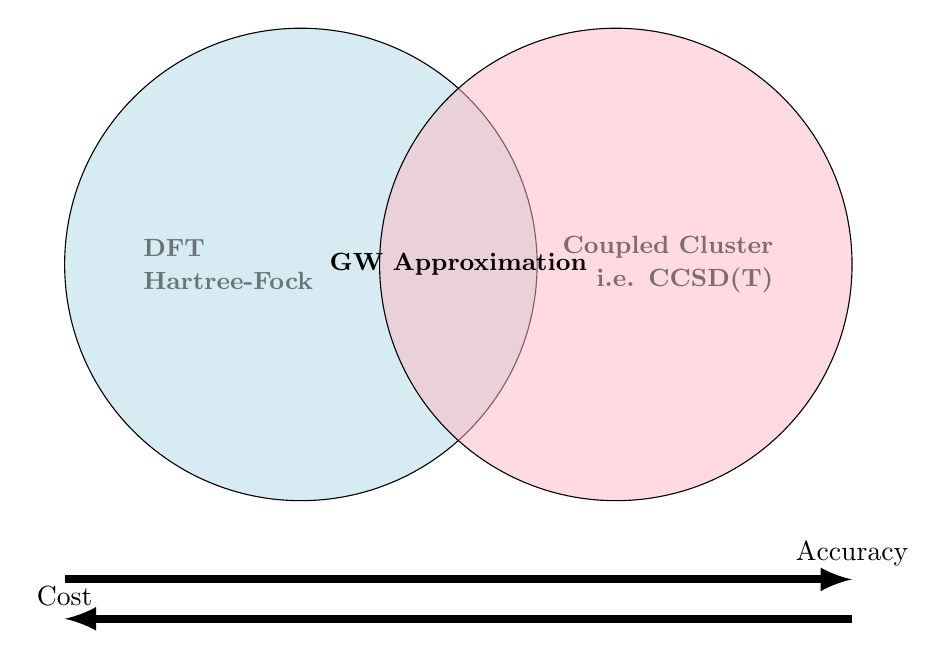
\begin{tikzpicture}
        % Define colors for the Venn diagram
        \definecolor{lowcolor}{RGB}{173,216,230}
        \definecolor{highcolor}{RGB}{255,182,193}

        % Draw the two overlapping circles
        \draw[fill=lowcolor, fill opacity=0.5] (-2, 0) circle (3cm) node [text width=4cm, align=left] {\small \textbf{DFT}\\ \textbf{Hartree-Fock}};
        
        \draw[fill=highcolor, fill opacity=0.5] (2, 0) circle (3cm) node [text width=4cm, align=right] {\small \textbf{Coupled Cluster}\\ \textbf{i.e. CCSD(T)}};
        
        % Place the GW Approximation text without a circle
        \node at (0, 0) [text width=4cm, align=center] {\small \textbf{GW Approximation}};

        % Draw bold and larger arrows
        \draw[ultra thick, ->, >=latex, line width=1mm] (-5, -4) -- (5, -4) node[right, above] {Accuracy};
        \draw[ultra thick, <-, >=latex, line width=1mm] (-5, -4.5) -- (5, -4.5) node[pos=0, above] {Cost};

    \end{tikzpicture}


\end{frame}





\begin{frame}
    \frametitle{\textcolor{caltechorange}{Self-Energy}}
    \begin{figure}
        \caption{Electron gas propagation\autocite{mattuck_guide_1992}}
        \begin{subfigure}{.4\textwidth}
            \centering
            \includegraphics[width=.8\linewidth]{shot.png}
            \caption{The \textbf{bare} electron is shot into the gas}
            \label{fig:shot}
        \end{subfigure}
        \begin{subfigure}{.4\textwidth}
            \centering
            \includegraphics[width=.8\linewidth]{clothing.png}
            \caption{The \textbf{quasi}-electron dynamically creates holes}
            \label{fig:clothing}
        \end{subfigure}
        \label{fig:propagates}
    \end{figure}
\pause
    Qualitatively 
    \begin{equation}
        \highlight{\epsilon_{\text{self}} = \epsilon_{\text{quasi}} - \epsilon_{\text{bare}},}
    \end{equation}
    The \textbf{self-energy} $\Sigma $ can be thought of as the difference between the quasi and bare electron
\end{frame}



\begin{frame}
    \frametitle{\textcolor{caltechorange}{$G_0W_0$ iterative procedure \autocite{bruneval_assessment_2019} for $\varepsilon_{p}^{\mathrm{QP}}$}}
    \begin{equation}
\highlight{\epsilon_p^{\mathrm{MF}} + \Sigma_p^{\mathrm{corr}}(\varepsilon_p^{\mathrm{QP}}) = \varepsilon_p^{\mathrm{QP}}}
    \end{equation}
    \begin{enumerate}
        \item start with the mean-field guess $\epsilon_p^{\mathrm{MF}}$
        \item add self-energy, evaluated at $\varepsilon_p^{\mathrm{QP}}$ from the previous iteration
        \item iterate until self-consistency in $\varepsilon_p^{\mathrm{QP}}$ is reached
    \end{enumerate}

\end{frame}
\begin{frame}
    \frametitle{\textcolor{caltechorange}{Linearized $G_0W_0$ density matrix\autocite{bruneval_assessment_2019}:}}
\textbf{Natural occupations}:  number of electrons in a given orbital.\autocite{szabo_modern_2012}
\begin{figure}[h]
    \includegraphics[width=0.9\textwidth]{h2_occupations.png}
\caption{HOMO and LUMO of $\mathrm{H_2}$ along the dissociation coordinate}

\end{figure}
\end{frame}









\begin{frame}
    \frametitle{\textcolor{caltechorange}{Bibliography}}
    \printbibliography
\end{frame}

\end{document}
